%! Author = joel
%! Date = 14.6.2020

% Preamble
\documentclass[11pt]{book}

% Packages
\usepackage{amsmath}
\usepackage{guitarchordschemes}
\usepackage{guitar}
\usepackage{graphicx}
\title{My chords, scales and songs that I have learned}
\author{Joel Sågfors}
\date{\today}
% Document
\makeindex
\begin{document}
    \maketitle


    \chapter{Introduction}
    This is my personal reference on all music related topics on the guitar.
    As the title states, this work will contain chords, scales and songs.


    \section{Music Theory}
    Notes are just sound waves of certain frequencies that are named by letters, and for the mostpart something inbetween the letters.
    It is like the compass, we have north, south, east and west.
    North-west in between north and west and so forth.
    In music you have sharp ($\sharp$) and flat ($\flat$), which is one semitone higher and lower, respectively.
    Except between E and F there is no "middle note".
    The same goes for B and C.
    This is illustrated in figure \ref{fig:note_circle}

    \begin{figure}[h]
        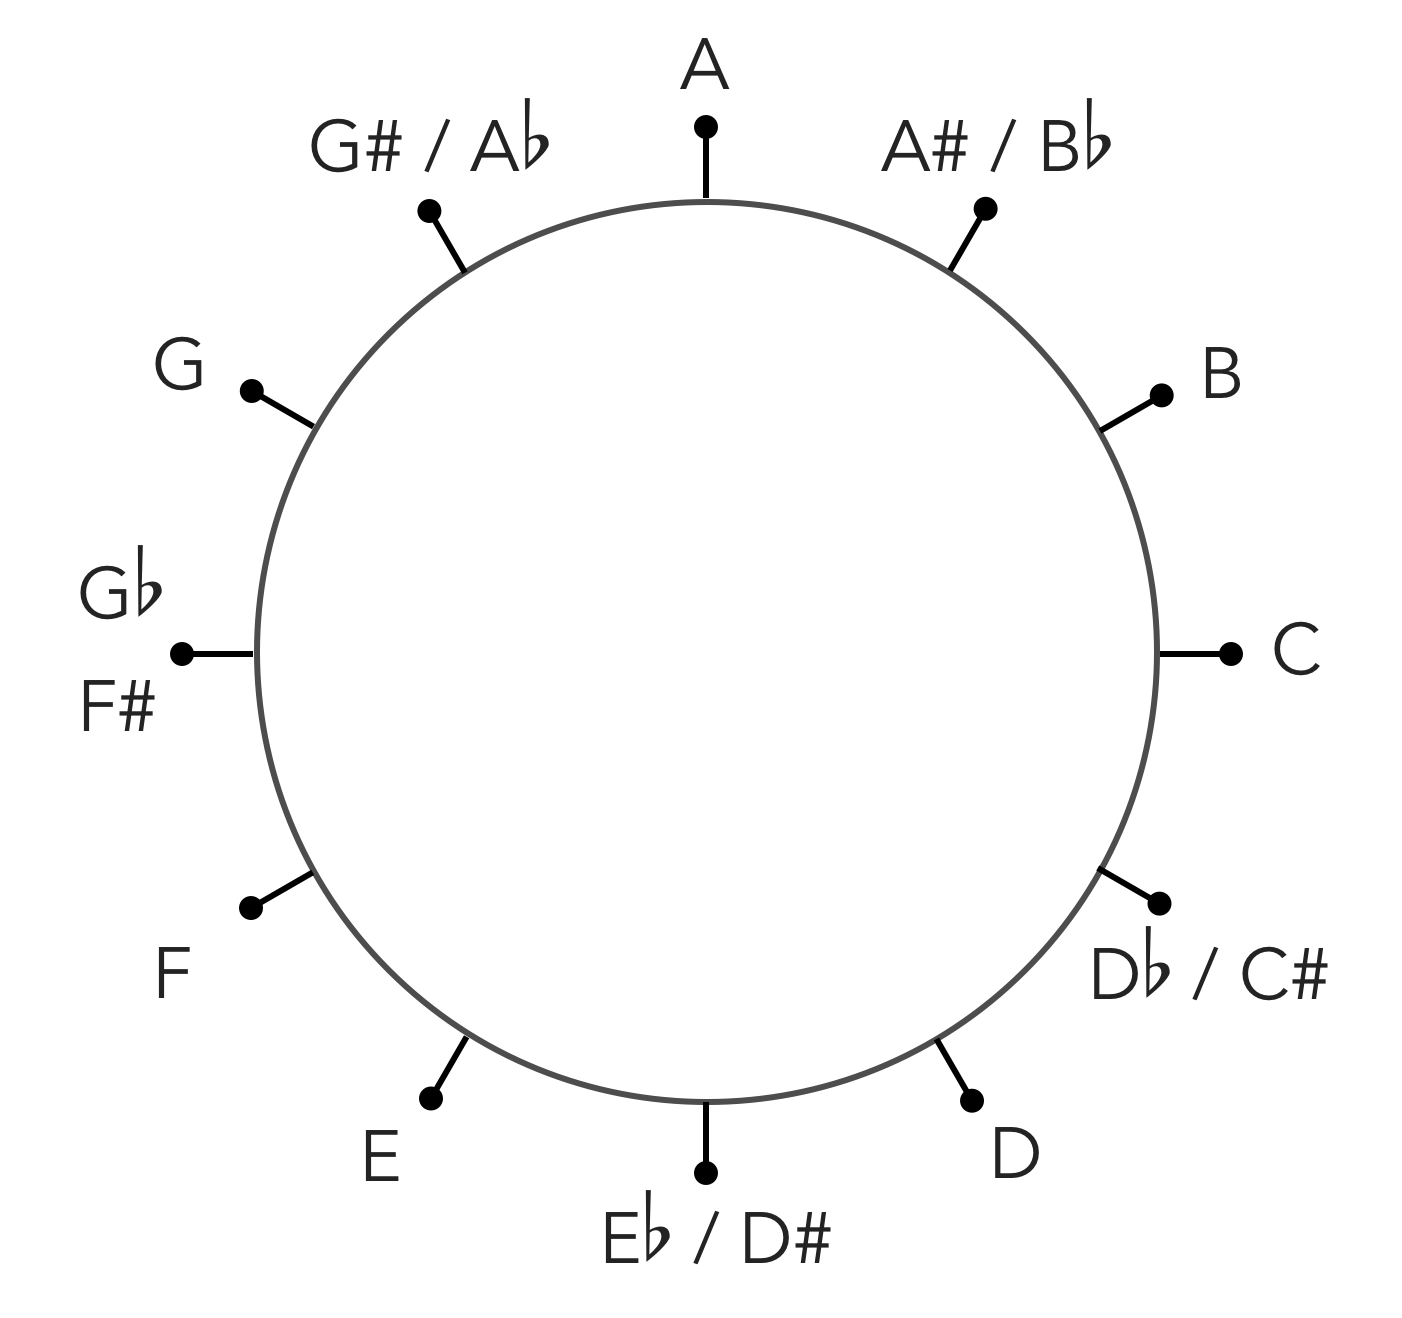
\includegraphics[width=\textwidth]{note_circle.png}
        \caption{The note circle, courtesy of Justin Sandercoe}
        \label{fig:note_circle}
    \end{figure}


    \chapter{Chords}
    Learning chords is a cornerstone to learning guitar.
    Strumming chords is usually the first way a beginner plays the guitar.
    In this chapter we explore the different chords for each note as I learn them, starting from the open major chord.


    \section{A chord}
    Starting from the first letter in the alphabet, the A chord is also one of the first chords that a guitar player learns,
    and is used in a lot of songs.

    \subsection{Open A major}
    This chord is easier to play with the fingers "out-of-order" as listed in the chord-box.
    The fingering makes it easier to get all fingers close to the fret.
    The root is in the fifth string.

    \chordscheme[
    name   = A,
    finger = {2/4:2,2/3:1,2/2:3},
    ring   = {5,1},
    mute   = {6}
    ]

    The notes in this chord is, A, E, A, C\#, E

    \subsection{A minor}
    Pretty self-explanatory, the minor version of A.

    \chordscheme[
    name = Am,
    finger = {2/4:2, 2/3:3, 1/2:1},
    ring = {5,1},
    mute = {6}
    ]

    The notes in this chord are A, E, A, C, E.

    \subsection{Asus2}
    The sus in the name comes from suspended, we suspend (remove) the third in the chord.
    The gist of it is that we create major chords from the 1st, 3rd, and 5th notes in a key.
    This third note plays an important part in the chords, when it is flattened by a semitone, we get a minor chord.
    When removing it altogether we get a suspended chord.

    Numbering the suspended chords follows its own logic.
    The number corresponds to the note that has replaced the 3rd, in this case it is replaced by the 2nd note in A scale.
    The third note in A is C\#, in this case replaced by B.
    The fingering here is not set in stone, since it can be a bit weird to stretch the finger down to the 3rd fret some alternative is fine.


    \chordscheme[
    name = Asus2,
    finger = {2/4:2,2/3:3},
    mute = {6},
    ring = {5,2,1}
    ]

    The notes in this chord are A, E, A, B, E.

    \subsection{Asus4}
    Another variant of Asus.
    This time C\# is raised to D.

    \chordscheme[
    name = Asus4,
    finger = {2/4:2, 2/3:3, 3/2:(3/4)},
    mute = {6},
    ring = {5,1}
    ]

    The notes in this chord are A, E, A, D, E.

    \subsection{A7}
    "Seventh" chords are used much in blues, the name comes from the seventh note in the scale.

    \chordscheme[
    name = A7,
    finger = {2/4:2, 3/2:4},
    mute = {6},
    ring = {5,3,1}
    ]


    \section{B chord}
    'Open B' is not regularly taught to beginners, my guess is that it is considered hard.
    However, barre B is pretty easy if you know barre F.

    \subsection{B7}
    A blues chord that is also used in for example in 'I Wanna Hold Your Hand' by The Beatles.

    \chordscheme[
    name = B7,
    finger = {2/5:1, 1/4:2, 2/3:3, 2/1:4},
    mute = {6},
    ring = {2}
    ]


    \section{D chord}
    An easy chord that has a chirpy sound because we don't play the two lowest strings at all.

    \chordscheme[
    name = D,
    finger = {2/3:1, 3/2:3, 2/1:2},
    ring = {4},
    mute = {6,5}
    ]

    Notes in this chord are D, A, D, F\#.

    \subsection{D minor}
    I have always struggled with the fingering of this chord, hope to get it one day.

    \chordscheme[
    name = Dm,
    finger = {2/3:2, 3/2:3, 1/1:1},
    ring = {4},
    mute = {5,6}
    ]

    Notes in this chord are D, A, D, F, which means F\# is the third in D.


    \section{F chord}
    The second to last note in the note circle, and a dreaded chord for many beginners, because the 'normal' version of
    F is barre.
    With proper practice you can however learn the barred version and in the process you learned a lot of chords as this shape can be moved around.

    \subsection{Barre F}

    \chordscheme[
    name = F,
    finger = {3/5:4,3/4:4,2/3:2},
    barre = {1/1-6:1}
    ]


    \chapter{Scales}


    \section{Minor Pentatonic}
    One of, if not the most common scales in rock and blues music is the minor pentatonic scale.
    The name means minor five note scale and that is pretty much what it is.
    The beauty of the minor pentatonic scale is that it can be played anywhere on the guitar neck, which makes it very versatile.

    The basis of the scale goes as follows:

    \bigskip

    \scales[
    name = Minor Pentatonic,
    finger = {
    2/1:1, 5/1:4,
    2/2:1, 5/2:4,
    2/3:1, 4/3:3,
    2/4:1, 4/4:3,
    2/5:1, 4/5:3,
    2/6:1, 5/6:4
    },
    root = {2/6, 4/4, 2/1}
    ]


    \section{Major Scales}
    Major scales are for the major notes in the circle.
    I learned this is primary school but has since needed to relearn

    \subsection{C Major}
    The first major scale I learned for guitar was C Major.
    It consists of only major notes and can be played from the top of the neck, where I learned.

    \scales[
    name = C Major
    position = 1,
    finger = {
    1/1:1,3/1:3,
    1/2:1,3/2:3,
    2/3:2,
    2/4:2,3/4:3,
    2/5:2,3/5:3,
    1/6:2,3/6:3
    }
    ]

    \subsubsection{Chords in C Major}
    These are the chords in C:

    C, Dm, Em, F, G, Am

    Numbered like.

    1 = C
    2 = Dm
    3 = Em
    4 = F
    5 = G
    6 = Am


    \chapter{Songs}


    \section{Californication - Red Hot Chili Peppers}
    One of the "easier" songs around that still provide something outside the normal chord strumming.
    This is the first song that I attempt to write down in this book,it has taken some time to master it but daily practice does a lot.

    \subsection{Riff}
    The riff is played throughout the verse, and the original version is fairly easy.
    I will show both this easier version, and a modified version that includes the bass part which is nice to play if one is doing it solo.


\end{document}